Over the last decade, use of web and thick client applications globally has greatly increased.
People increasingly access services online--to manage their finances \citep{jayawardhena2000changes}, use government
services \citep{fox2010directgov} and communicate using social media \citep{boulianne2015social}.
On a daily basis users entrust these systems with maintaining the privacy of their personal information and safeguarding
their finances.
With the transition from a web centred primarily around exchanging documents to a platform for deploying complex
applications, security is increasingly important.

\section{Application Security}

Application security is of particular interest because it transcends the underlying infrastructure on which applications
are deployed.
Despite the popularity of cloud IaaS (infrastructure-as-a-service) and PaaS (platform-as-a-service)
offerings which can substantially improve infrastructure security, applications will continue to be vulnerable.

The predominant cause of these vulnerabilities is improper user input handling \citep{schneier2011secrets}.
The \emph{Open Web Application Security Project} (OWASP) regularly publishes a list of the top ten most critical
security issues, and a subset of these are described below \citep{owasp10}:

\begin{description}
    \item[Injection] Covers query injection, where user input is improperly interpolated into a e.g. database Structured
                     Query Language (SQL) query or a directory LDAP search. Malicious user input can retrieve or modify
                     sensitive data, bypass authorisation controls and (in some cases) run arbitrary code \citep[p.~291]{stuttard2011web}.
    \item[Broken Access Control] Covers vulnerabilities such as insecure direct object access (IDOR) where authorisation
                                 checks are not implemented consistently and the user's request is trusted in one or
                                 more parts of the application \citep[p.~257]{stuttard2011web}. Also includes path
                                 traversal vulnerabilities where user input is used to construct a filesystem path and a
                                 malicious actor can include e.g. \texttt{../} to traverse up one level.
    \item[XML External Entities (XXE)] A vulnerability which involves improperly handling user encoded in the XML
                                       interchange format. XML supports functionality to reference entities from an
                                       external location. Exploitation may allow arbitrary files to be read, sensitive
                                       data to be exposed or code to be executed  \citep[p.~384]{stuttard2011web}.
    \item[Cross-Site Scripting (XSS)] When user input is not properly handled in the context of a HTML web page or
                                      inside JavaScript, a user can provide malicious input that can run arbitrary code
                                      on the client. This can be used by an attacker to steal or misuse a victim's
                                      session \citep[p.~431]{stuttard2011web}.
    \item[Insecure Deserialization] Results from insecurely converting user input into a language object.
\end{description}

Many of these vulnerabilities--and the necessary techniques for preventing them--have been well-established for a
number of years, and yet they continue to be regularly discovered in production applications \citep[p.~2]{schneier2011secrets}.

\subsection{Examples}\label{subsec:examples}

From the above classes of vulnerabilities, we will focus on a subset of motivating examples.
In the context of a Java Enterprise Edition (EE) application these will include SQL injection, LDAP injection and
path traversal.

\subsubsection{SQL Injection}
\label{ex:sqli}

Structured Query Language (SQL) is used with relational database systems to create, retrieve, update and delete data.
SQL injection falls into the \emph{injection} category of vulnerabilities above.
Generally, it arises when SQL queries concatenate or interpolate user input into a query command.
An attacker is able to craft user input that ``breaks out'' of e.g. a string literal and execute arbitrary SQL.
This could lead to exfiltration of sensitive data, destruction of data or violation of data integrity.
SQL injection is typically mitigated using \emph{prepared statements} \citep{stuttard2011web}, which allow placeholders to be set-up in the
query and then bound to meaningful values at execution time.
By using this technique to bind user input to specific placeholders, the possibility to inject SQL is removed.

The example below shows a Java function, \texttt{lookupUserNameByToken}, which performs a query to retrieve data from
a \textsc{Users} table based on a user-provided \texttt{token} argument.
Instead of using a prepared statement, once the query is created, the token input is concatenated directly into the
\textcolor{id7-aubergine}{where} clause.

\newsavebox\myv

\begin{lrbox}{\myv}\begin{minipage}{\textwidth}
\begin{minted}[fontsize=\fontsize{0.01pt}{0.01pt}]{java}
public String lookupUserNameByToken(String token) throws SQLException {
    Statement stmt = connection.createStatement();
    String query = "select * from Users where ";
    query += "token = '" + token + "'";
    ResultSet rs = stmt.executeQuery(sql);
    if (rs.next()) {
        return rs.getString("name");
    }
    return null;
}
\end{minted}
\end{minipage}\end{lrbox}

\begin{mdframed}[backgroundcolor=lightgrey]
\begin{Verbatim}[commandchars=\\\{\}]
\PYGidseven{k+kd}{public} \PYGidseven{n}{String} \PYGidseven{n+nf}{lookupUserNameByToken}\PYGidseven{o}{(}\PYGidseven{n}{String} \PYGidseven{n}{token}\PYGidseven{o}{)} \PYGidseven{k+kd}{throws} \PYGidseven{n}{SQLException} \PYGidseven{o}{\PYGidsevenZob{}}
    \PYGidseven{n}{Statement} \PYGidseven{n}{stmt} \PYGidseven{o}{=} \PYGidseven{n}{connection}\PYGidseven{o}{.}\PYGidseven{n+na}{createStatement}\PYGidseven{o}{(}\PYGidseven{o}{)}\PYGidseven{o}{;}
    \PYGidseven{n}{String} \PYGidseven{n}{query} \PYGidseven{o}{=} \PYGidseven{l+s}{\PYGidsevenZdq{}select * from users where \PYGidsevenZdq{}}\PYGidseven{o}{;}
    \colorbox{id7-ruby-red}{\textcolor{white}{\faExclamationTriangle{} \PYGidseven{n}{query} \PYGidseven{o}{+=} \PYGidsevenZdq{} token = '\PYGidsevenZdq{} \PYGidseven{o}{+} \PYGidseven{n}{token} \PYGidseven{o}{+} \PYGidsevenZdq{}'\PYGidsevenZdq{} \PYGidseven{o}{;}}}
    \PYGidseven{n}{ResultSet} \PYGidseven{n}{rs} \PYGidseven{o}{=} \PYGidseven{n}{stmt}\PYGidseven{o}{.}\PYGidseven{n+na}{executeQuery}\PYGidseven{o}{(}\PYGidseven{n}{sql}\PYGidseven{o}{)}\PYGidseven{o}{;}
    \PYGidseven{k}{if} \PYGidseven{o}{(}\PYGidseven{n}{rs}\PYGidseven{o}{.}\PYGidseven{n+na}{next}\PYGidseven{o}{(}\PYGidseven{o}{)}\PYGidseven{o}{)} \PYGidseven{o}{\PYGidsevenZob{}}
        \PYGidseven{k}{return} \PYGidseven{n}{rs}\PYGidseven{o}{.}\PYGidseven{n+na}{getString}\PYGidseven{o}{(}\PYGidseven{l+s}{\PYGidsevenZdq{}name\PYGidsevenZdq{}}\PYGidseven{o}{)}\PYGidseven{o}{;}
    \PYGidseven{o}{\PYGidsevenZcb{}}
    \PYGidseven{k}{return} \PYGidseven{k+kc}{null}\PYGidseven{o}{;}
\PYGidseven{o}{\PYGidsevenZcb{}}
\end{Verbatim}
\end{mdframed}

An attacker able to directly specify a token, could provide an input string containing a single quote \texttt{'}
character to break out of the string literal in the query.

For instance, providing a token \texttt{' or 1=1 --} would create the following query:

\begin{minted}{sql}
select * from Users where token = '' or 1=1 -- '
\end{minted}

\infobox{
The \texttt{--} token is used to create a comment until the end of the query.
This ensures no syntax error is introduced when the Java code ends the string after appending the user input.}

This query would return all users in the database.

\subsubsection{LDAP Injection}

The Lightweight Directory Access Protocol (LDAP) is a networked protocol designed for querying directory services.
These services are used for storing and organising network entities, such as users and devices.
Microsoft's Active Directory (AD) is a commonly deployed enterprise solution for storing user information and handling
network authentication.

\begin{figure}[H]
    \begin{MyMdframed}
        \vspace{0.5em}


        \caption{\label{figure:wso}LDAP is used internally at Warwick to power the single sign-on system}
        \vspace{0.5em}
        \captionsetup{style=default}
        \begin{center}
            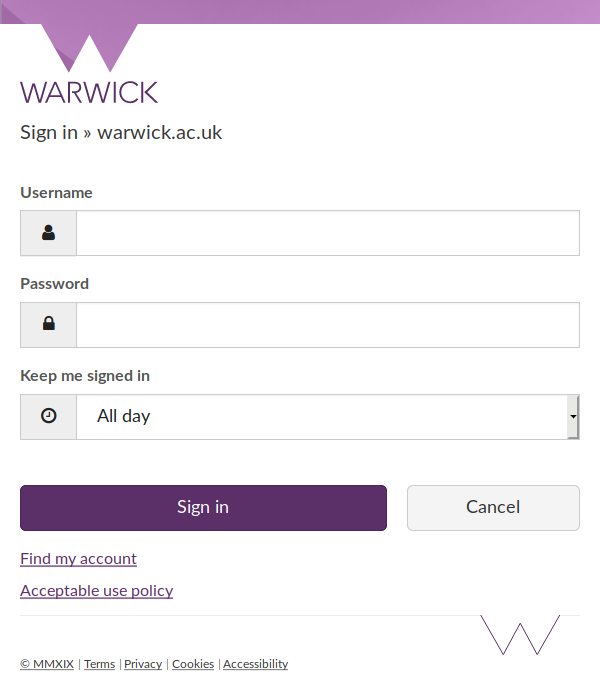
\includegraphics[width=0.5\linewidth]{wso.png}
        \end{center}
    \end{MyMdframed}
\end{figure}

LDAP queries are written in a compact manner using symbols for each operation and parentheses for each clause:

\texttt{(\&(warwickUniId=1510654)(sn=Williams))}

This query retrieves the user with attribute \texttt{warwickUniId} set to value 1510654 \emph{and} surname (sn) set to value
``Williams''.
The \texttt{\&} operator specifies conjunction to be applied to the nested filters.

Much like SQL injection, LDAP injection arises when user-input is concatenated into a filter name or value:

\newsavebox\myva
\begin{lrbox}{\myva}\begin{minipage}{\textwidth}
    \begin{mycodefile}{csharp}{\label{code:motivating:ldap:1}A vulnerable LDAP query function}{C\#}{ldap.cs}\end{mycodefile}
\end{minipage}\end{lrbox}

\begin{mdframed}[backgroundcolor=lightgrey]
\begin{Verbatim}[commandchars=\\\{\}]
\PYGidseven{k}{public} \PYGidseven{k+kt}{string} \PYGidseven{n+nf}{GetSurnameForUser}\PYGidseven{p}{(}\PYGidseven{k+kt}{string} \PYGidseven{n}{username}\PYGidseven{p}{)}
\PYGidseven{p}{\PYGidsevenZob{}}
    \PYGidseven{k+kt}{var} \PYGidseven{n}{directoryEntry} \PYGidseven{p}{=} \PYGidseven{k}{new} \PYGidseven{n}{DirectoryEntry}\PYGidseven{p}{(}\PYGidseven{l+s}{\PYGidsevenZdq{}LDAP://acme.corp\PYGidsevenZdq{}}\PYGidseven{p}{);}
    \PYGidseven{k+kt}{var} \PYGidseven{n}{searcher} \PYGidseven{p}{=} \PYGidseven{k}{new} \PYGidseven{n}{DirectorySearcher}\PYGidseven{p}{(}\PYGidseven{n}{directoryEntry}\PYGidseven{p}{);}
    \colorbox{id7-ruby-red}{\textcolor{white}{\faExclamationTriangle{} searcher.Filter = \PYGidsevenZdq{}(cn=\PYGidsevenZdq{} + username + \PYGidsevenZdq{})\PYGidsevenZdq{};}}
    \PYGidseven{k+kt}{var} \PYGidseven{n}{result} \PYGidseven{p}{=} \PYGidseven{n}{searcher}\PYGidseven{p}{.}\PYGidseven{n}{FindOne}\PYGidseven{p}{();}
    \PYGidseven{k}{return} \PYGidseven{n}{result}\PYGidseven{p}{.}\PYGidseven{n}{Properties}\PYGidseven{p}{[}\PYGidseven{l+s}{\PYGidsevenZdq{}sn\PYGidsevenZdq{}}\PYGidseven{p}{][}\PYGidseven{l+m}{0}\PYGidseven{p}{].}\PYGidseven{n}{ToString}\PYGidseven{p}{();}
\PYGidseven{p}{\PYGidsevenZcb{}}
\end{Verbatim}
\end{mdframed}

The impact is generally more limited, but due to the support for wildcard characters it is possible to leak other
attribute values by testing for a character at a time.
Numeric values or dates can be exfiltrated using a binary search approach.

\begin{figure}[H]
    \begin{MyMdframed}
        \vspace{0.5em}


        \caption{Injection into a conjunctive query can be used to exfiltrate data}
        \vspace{0.5em}
        \captionsetup{style=default}

        \begin{center}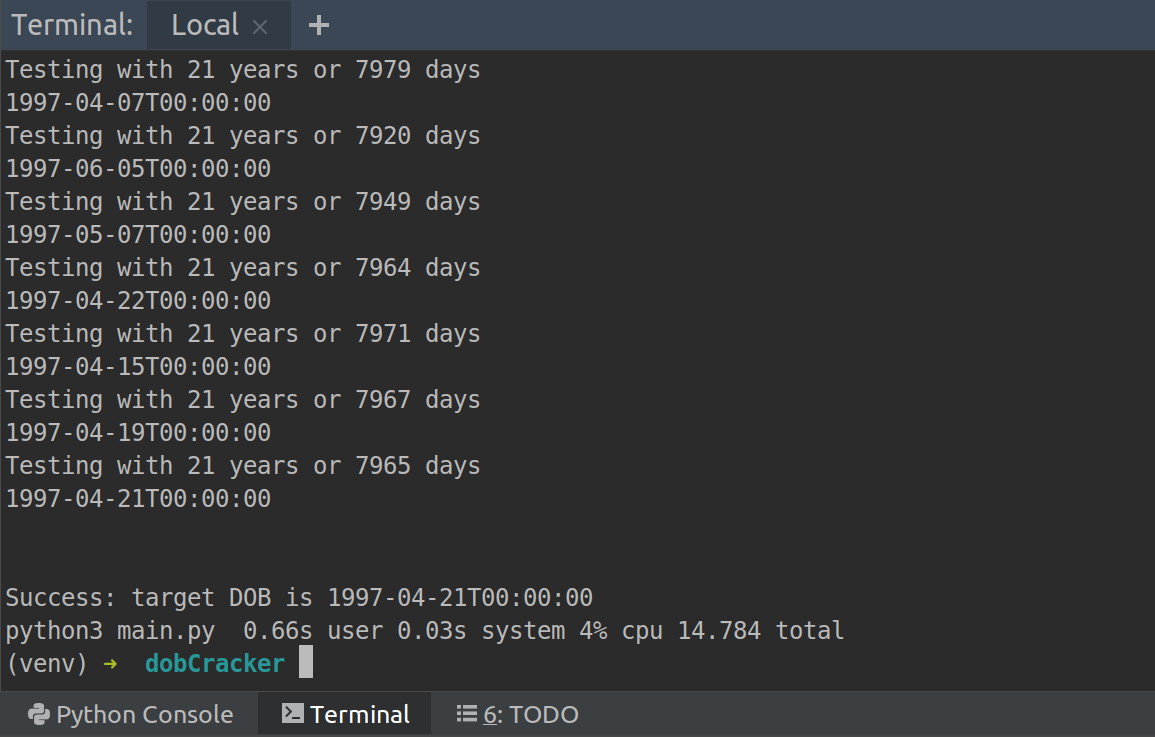
\includegraphics[width=0.5\linewidth]{dobcrack.png}\end{center}

        \vspace{0.5em}

        Note that despite network latency, we can still leak a value in a short period of time (< 15s) by
        repeatedly querying an oracle with less than/greater than filters and observing the response.
    \end{MyMdframed}
\end{figure}

The best practice for mitigating this vulnerability involves using an encoder that is able to escape LDAP control
characters (for example, right parenthesis is replaced with \texttt{\textbackslash 29}).
This ensures that user input is then not considered part of a query.

\subsubsection{Path Traversal}

Many applications read and write files to the filesystem.
Problems arise when user input is permitted to influence the destination path.

Consider a Java function which is designed to persist user preference information in a text file:

\newsavebox\myvb
\begin{lrbox}{\myvb}\begin{minipage}{\textwidth}
\begin{mycodefile}{java}{Hidden}{Java}{pathtraversal.java}\end{mycodefile}
\end{minipage}\end{lrbox}

\begin{mdframed}
\begin{Verbatim}[commandchars=\\\{\}]
\PYGidseven{k+kd}{public} \PYGidseven{k+kd}{static} \PYGidseven{k+kt}{void} \PYGidseven{n+nf}{writeUserPreference}\PYGidseven{o}{(}\PYGidseven{n}{String} \PYGidseven{n}{username}\PYGidseven{o}{,} \PYGidseven{n}{Preference} \PYGidseven{n}{pref}\PYGidseven{o}{)} \PYGidseven{o}{\PYGidsevenZob{}}
    \PYGidseven{k}{try} \PYGidseven{o}{\PYGidsevenZob{}}
        \colorbox{id7-ruby-red}{\textcolor{white}{\faExclamationTriangle{} String path = \PYGidsevenZdq{}/tmp/prefs/\PYGidsevenZdq{} + username;}}
        \PYGidseven{n}{Files}\PYGidseven{o}{.}\PYGidseven{n+na}{writeString}\PYGidseven{o}{(}\PYGidseven{n}{Paths}\PYGidseven{o}{.}\PYGidseven{n+na}{get}\PYGidseven{o}{(}\PYGidseven{n}{path}\PYGidseven{o}{),} \PYGidseven{n}{pref}\PYGidseven{o}{.}\PYGidseven{n+na}{toString}\PYGidseven{o}{());}
    \PYGidseven{o}{\PYGidsevenZcb{}} \PYGidseven{k}{catch}\PYGidseven{o}{(}\PYGidseven{n}{IOException} \PYGidseven{n}{e}\PYGidseven{o}{)} \PYGidseven{o}{\PYGidsevenZob{}}
        \PYGidseven{n}{e}\PYGidseven{o}{.}\PYGidseven{n+na}{printStackTrace}\PYGidseven{o}{();}
    \PYGidseven{o}{\PYGidsevenZcb{}}
\PYGidseven{o}{\PYGidsevenZcb{}}
\end{Verbatim}
\end{mdframed}

If a user is able to influence the username passed as an argument to the function and choose a malicious name, such as
the string \texttt{../../etc/ssh/sshd_config}, they will be able to write to files on the filesystem outside of the
location which the developer intended.
This issue can arise with both write and read operations.
Depending on which files are available to the application, this vulnerability can lead to a full system compromise.

Path traversal vulnerabilities have been reported in software for at least 20 years but still regularly make appearances
in modern applications.
As an example, CVE-2019-1002101 was disclosed in March 2019.
This vulnerability impacts Kubernetes, a popular container orchestration system developed by Google.
The root cause is a directory traversal vulnerability arising due to the system trusting unsafe input from an archive
file.

\section{Static Analysis}

Static analysis tools can detect some classes of vulnerability by examining source code.
Within application security, static analysis tools are grouped under the \emph{Static Application Security Testing} SAST
denomination in contrast to \emph{Dynamic Application Security Testing} (DAST) tools which operate at runtime and
observe the behaviour of a running system.
SAST tools work by either independently parsing the developer's code or
analysing an \emph{abstract syntax tree} (AST) produced by the language toolchain\footnote{%
    In the context of C\#, Microsoft have made the \emph{Roslyn} compiler source code available and many static analysis
    tools are built on top of this open platform.}
and using a series of inspections to check and log common problems.
Some more advanced tools use \emph{taint tracking} combined with information flow analysis to mark and track variables
and parameters that have been influenced by user input \citep{denning1977certification}.
Functions or procedures for which it is dangerous to receive user input are marked as \emph{taint sinks}, whereas
sources of user input are known as \emph{taint sources}.
A list of sinks that are deemed potentially dangerous (such as database query functions) is maintained, and user input
flowing to any of these sinks results in an issue being logged.

For the example discussed in section \ref{ex:sqli}, the \texttt{token} argument would be marked as a
\emph{taint source}; this indicates that it is either completely or partially influenced by user input.
The \texttt{executeQuery} method on the \texttt{java.sql.Statement} class instance would, in contrast, be recognised
as a sink.

As discussed in \citet{sadowski2018lessons}, it is preferable to detect issues in a static fashion--ideally integrated
into the build process--to ensure that problems are actioned by developers.
The false positive rate should also be minimised to avoid the risk of \emph{alert fatigue},a problem which occurs in a
variety of different contexts where the value of alerts is decreased due to a perception that often, there is no real
substance to the warnings \citep{kesselheim2011clinical}.

If reliable and properly implemented, static analysis tooling has been shown to be able to prevent whole classes of
bugs from making it into production \citep{sadowski2018lessons}.

\section{A Better Approach}

Existing static analysis are often unable to evaluate the effectiveness of input validation code that may already be in
place--leading to false positives.
This is because the tools consider code in isolation and cannot reason about the form of user input.
Taint tracking is similarly ``binary'', where data originates from user input and is assumed dangerous or originates
elsewhere and assumed benign.

We describe a system which uses \emph{refinement types} in order to determine whether existing regular expression based
input validation is effective.
This happens at compile time, using an SMT solver to find situations where input could fail to be matched by a regular
expression.
This allows for potential security issues to be surfaced during type-checking.

Our work meets the follow formal objectives (first described in appendix \ref{project:spec}):

\begin{enumerate}
    \item Formalise a type system that supports types predicated with a regular expression pattern that elements of the refined type will satisfy (be matched by).
    \begin{enumerate}
        \item Explore the consequences of typical string operations (e.g. concatenation) and define the type of
        their return value when applied to elements of the regular expression type.

        \item At minimum, this should allow for simple functions to be declared that can safely accept/return a
        particular regular expression input.
        \item Evaluate the rate of false positives when compared to existing static analysis
    \end{enumerate}
    \item Implement such a type system that can guarantee type safety, built against a simplified proof-of-concept
    language.
    \begin{enumerate}
        \item Test the implementation against a variety of test cases. The testing strategy should make use of
        automated unit tests, and manual system testing considering both general expected input as well as
        any relevant ``edge-cases'' that need to be handled.
    \end{enumerate}
\end{enumerate}

We know of no existing program verification tools capable of verifying regular expression membership properties
within a programming language using pre/post-conditions or type annotations--our system is novel in this respect.
Section \ref{sec:prior-art} discusses some of the existing static analysis tooling and languages that have been
developed in more depth.